%
% cauchy.tex
%
% (c) 2021 Prof Dr Andreas Müller, OST Ostschweizer Fachhochschule
%
\section{Cauchy-Integral
\label{buch:funktionentheorie:section:cauchy}}
\rhead{Cauchy-Integral}
In Abschnitt~\ref{buch:funktionentheorie:section:holomorph} hat sich
bereits gezeigt, dass komplexe Differenzierbarkeit einer komplexen
Funktion weit mehr Einschränkungen auferlegt als reelle Differenzierbarkeit.
Sowohl der Real- wie auch der Imaginärteil müssenharmonische Funktionen
sein.
In diesem Abschnitt wird die Cauchy-In\-te\-gral\-formel etabliert, die 
sogar zeigt, dass eine komplex differenzierbare Funktion bereits durch 
die Werte auf dem Rand eines einfach zusammenhängenden Gebietes
gegeben ist, beliebig oft differenzierbar ist und ausserdem immer
analytisch ist.

%
% Wegintegrale und die Cauchy-Formel
%
\subsection{Wegintegrale\label{subsection:wegintegrale}}
Das Finden einer Stammfunktion, die Integration, ist die Grundtechnik,
\index{Stammfunktion}%
mit der man den Übergang von lokaler Information in Form von Ableitungen,
zu globaler Information über reelle Funktionen vollzieht.
Sie liefert aus der Steigung zwischen zwei Punkten $x_0$ und $x$ den
Funktionswert mittels
\[
f(x)=f(x_0)+\int_{x_0}^xf'(\xi)\,d\xi.
\]
Bei einer reellen Funktion gibt es nur eine Richtung, entlang der man
integrieren könnte.

Auch in der komplexen Ebene erwarten wir eine Formel
\[
f(z) = f(z_0) + \int_{z_0}^z f'(\zeta)\,d\zeta.
\]
In der komplexen Ebene gibt es aber beliebig viele Wege, mit denen die
Punkte $z_0$ und $z$ verbunden werden können.
Der Wert von $f(z)$ muss also durch Integration entlang eines speziell
gewählten Weges $\gamma$
\[
f(z) = f(z_0) + \int_{\gamma} f'(\zeta)\,d\zeta
\]
bestimmt werden.
Es muss also zunächst geklärt werden, wie ein solches Wegintegral
überhaupt zu verstehen und zu berechnen ist.
Dann gilt es zu untersuchen, inwieweit diese Konstruktion unabhängig
von der Wahl des Weges ist.
Für komplex differenzierbare Funktionen wird sich eine sehr erfolgreiche
Theorie ergeben.

%
% Wegintegrale
%
\subsubsection{Definition des Wegintegrals}
Ein Weg in der komplexen Ebene ist eine Abbildung
\index{Abbildung}%
\[
\gamma\colon [a,b]\to\mathbb C: t\mapsto \gamma(t).
\]
Wir verlangen für unsere Zwecke zusätzlich, dass $\gamma$ differenzierbar
ist.
Dann können wir für jede beliebige Funktion das Wegintegral definieren.

\begin{definition}
Sei $\gamma\colon[a,b]\to\mathbb C$ ein Weg in $\mathbb C$ und $f(z)$
eine stetige komplexe Funktion, dann heisst
\[
\int_{\gamma} f(z)\,dz = \int_a^bf(\gamma(t)) \gamma'(t)\,dt
\]
das {\em Wegintegral} von $f(z)$ entlang der Kurve $\gamma$.
\index{Wegintegral}
\end{definition}

\begin{beispiel}
Man berechne das Wegintegral der Funktion $f(z)=z^n$ entlang des
Weges
$\gamma(t)=1+t+it^2$
für $t\in[0,1]$.

Die Definition besagt
\begin{align*}
\int_\gamma f(z)\,dz
&=
\int_0^1 f(\gamma(t))\gamma'(t)\,dt
=
\int_0^1 \gamma(t)^n \gamma'(t)\,dt
=
\int_0^1 \frac{d}{dt}\frac{\gamma(t)^{n+1}}{n+1}\,dt
\\
&=
\biggl[\frac{\gamma(t)^{n+1}}{n+1}\biggr]_0^1
=
\frac{(2+i)^{n+1}}{n+1}-\frac{1^{n+1}}{n+1}
=
\frac{(2+i)^{n+1}-1}{n+1}.
\end{align*}
Man stellt in diesem Beispiel auch fest, dass das Integral offenbar
unabhängig ist von der Wahl des Weges, es kommt einzig auf die
beiden Endpunkte an:
\[
\int_\gamma z^n \,dz = \frac1{n+1}\bigl(\gamma(1)^{n+1}-\gamma(0)^{n+1}\bigr).
\]
\end{beispiel}

\begin{beispiel}
Wir berechnen als Beispiel das Wegintegral der Funktion $f(z)=1/z$ entlang
eines Halbkreises von $1$ zu $-1$.
Es gibt zwei verschiedene solche Halbkreise:
\begin{equation*}
\begin{aligned}
\gamma_+(t)&=e^{it},&t&\in[0,\pi]
\\
\gamma_-(t)&=e^{-it},&t&\in[0,\pi]
\end{aligned}
\end{equation*}
Wir finden für die Wegintegrale
\begin{align*}
\int_{\gamma_+}\frac1z\,dz
&=
\int_0^\pi \frac1{e^{it}}ie^{it}\,dt=i\int_0^\pi\,dt=i\pi,
\\
\int_{\gamma_-}\frac1z\,dz
&=
-\int_0^\pi \frac1{e^{-it}}ie^{-it}\,dt=-i\int_0^\pi\,dt=-i\pi.
\end{align*}
Das Wegintegral zwischen $1$ und $-1$ hängt also mindestens für diese
spezielle Funktion $f(z)=1/z$ von der Wahl des Weges ab.
\end{beispiel}

Wie Wahl der Parametrisierung der Kurve hat keinen Einfluss auf den
Wert des Wegintegrals.

\begin{satz}
\index{Satz!Kurvenparametrisierung}%
Seien $\gamma_1(t), t\in[a,b],$ und $\gamma_2(s),s\in[c,d]$
verschiedene Parametrisierungen
\index{Parametrisierung}%
der gleichen Kurve, es gebe also eine Funktion $t(s)$ derart, dass
$\gamma_1(t(s))=\gamma_2(s)$.
Dann ist
\[
\int_{\gamma_1}f(z)\,dz
=
\int_{\gamma_2}f(z)\,dz.
\]
\end{satz}

\begin{proof}[Beweis]
Wir verwenden die Definition des Wegintegrals
\begin{align*}
\int_{\gamma_1} f(z)\,dz
&=
\int_a^b f(\gamma_1(t))\,\gamma_1'(t)\,dt
=
\int_c^d f(\gamma_1(t(s))\,\underbrace{\gamma_1'(t(s)) t'(s)}_{\displaystyle
=\frac{d}{ds}\gamma_1(t(s))}\,ds
\\
&=
\int_c^d f(\gamma_2(s)\,\gamma_2'(s)\,ds
=
\int_{\gamma_2}f(z)\,dz.
\end{align*}
Beim zweiten Gleichheitszeichen haben wir die Formel für die
Variablentransformation $t=t(s)$ in einem Integral verwendet.
\index{Variablentransformation}%
\end{proof}

Wir erwarten, dass das Wegintegral ähnlich wie das Integral reeller
Funktionen eine Art ``Umkehroperation'' zur Ableitung ist.
Wir untersuchen daher den Fall, dass $f(z)$ eine komplexe Stammfunktion $F(z)$
hat, also $f(z)=F'(z)$.
Wir berechnen das Wegintegral entlang des Weges $\gamma$:
\begin{align*}
\int_{\gamma}f(z)\,dz
&=
\int_a^bf(\gamma(t))\,\gamma'(t)\,dt
=
\int_a^bF'(\gamma(t))\,\gamma'(t)\,dt
=
\int_a^b\frac{d}{dt}F(\gamma(t))\,dt
=
F(\gamma(a))-F(\gamma(b))
\end{align*}
Dies ist genau die Formel, die man als den Hauptsatz der Infinitesimalrechnung
kennt.
Trotzdem ist die Situation hier etwas anders.
In der reellen Infinitesimalrechnung war die Existenz einer Stammfunktion
durch das Integral gesichert, man konnte mit
\[
F(x)=\int_a^xf(\xi)\,d\xi
\]
immer eine Stammfunktion angeben.
Im komplexen Fall können wir natürlich auch versuchen, eine Stammfunktion
mit Hilfe von
\[
F(z)=\int_{\gamma_z} f(\zeta)\,d\zeta
\]
zu definieren.
Dabei muss allerdings $\gamma_z$ ein Weg sein, der im Punkt $z$ endet,
und wir wissen noch nicht einmal, ob die Wahl des Weges eine Rolle
spielt.
Bevor wir also sicher sein können, dass eine Stammfunktion existiert,
müssen wir zeigen, dass das Wegintegral einer komplex differenzierbaren
Funktion zwischen zwei Punkten nicht von der Wahl des Weges abhängt,
der die beiden Punkte verbindet.
Dazu ist notwendig, geschlossene Wege genauer zu betrachten.

%
% Wegintegrale führen auf analytische Funktionen
%
\subsubsection{Wegintegrale führen auf analytische Funktionen}
\begin{figure}
\centering
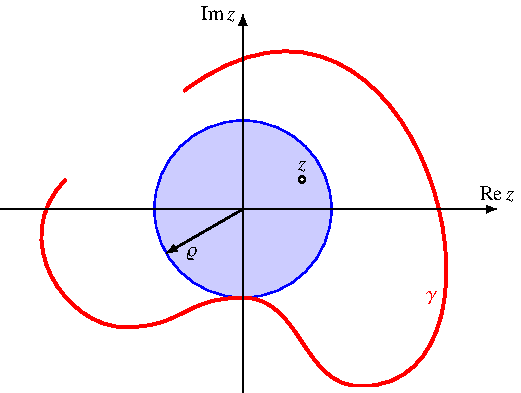
\includegraphics{chapters/080-funktionentheorie/images/integralanalytisch.pdf}
\caption{Pfad und Konvergenzradius für den Nachweis, dass Wegintegrale
auf analytische Funktionen führen (Satz~\ref{komplex:integralanalytisch}).
\label{komplex:integralanalytischpfad}}
\end{figure}
Mit Wegintegralen kann man aus stetigen Funktionen neue Funktionen
konstruieren.
Die folgende Konstruktion liefert überraschenderweise immer
analytische Funktionen.
\begin{satz}
\label{komplex:integralanalytisch}
Sei $\gamma\colon [a,b]\to\mathbb C$ ein Weg in $\mathbb C$, der nicht
durch den Nullpunkt verläuft, und $g$ eine stetige Funktion
auf $\gamma([a,b])$ (Abbildung~\ref{komplex:integralanalytischpfad}).
Dann ist die Funktion
\[
f(z) = \frac1{2\pi i}\int_\gamma \frac{g(x)}{x-z}\,dx
\]
in einer Umgebung des Nullpunktes analytisch:
\[
f(z) = \sum_{k=0}^\infty c_k z^k,\qquad
\text{mit\quad}
c_k=\frac1{2\pi i}\int_\gamma \frac{g(x)}{x^{k+1}}\,dx.
\]
Der Konvergenzradius $\varrho$ dieser Reihe ist der minimale Abstand der
Kurve $\gamma$ vom Nullpunkt.
\end{satz}

\begin{proof}[Beweis]
Zunächst schreiben wir
\begin{equation}
\frac{1}{x-z}
=
\frac1x\cdot \frac{1}{1-\displaystyle\frac{z}{x}}
=
\frac1x\cdot \sum_{k=0}^\infty \biggl(\frac{z}{x}\biggr)^k
=
\sum_{k=0}^\infty \frac{z^k}{x^{k+1}}.
\label{komplex:georeihe}
\end{equation}
Damit können wir jetzt die Funktion $f(z)$ berechnen:
\begin{align*}
f(z)
&=
\frac1{2\pi i} \int_{\gamma} \frac{g(x)}{x-z}\,dx
=
\frac1{2\pi i} \int_{\gamma} \sum_{k=0}^\infty \frac{z^k}{x^{k+1}}g(x)\,dx
=
\sum_{k=0}^\infty
\underbrace{\biggl(\frac1{2\pi i} \int_{\gamma} \frac{g(x)}{x^{k+1}}\,dx\biggr)}_{\displaystyle =c_k}
z^k
=
\sum_{k=0}^\infty c_kz^k.
\end{align*}
Wir müssen uns noch die Konvergenz dieser Reihen überlegen.
Wenn $z<\varrho$ ist, dann ist
\[
\biggl|\frac{z}{x}\biggr| 
=
\frac{|z|}{|x|}
<1,
\]
so dass die geometrische Reihe \eqref{komplex:georeihe} konvergent ist,
daraus lesen wir ab, dass der Konvergenzradius mindestens $\varrho$
ist.
Grösser kann er allerdings auch nicht sein, da für $|z|\ge \varrho$
das Integral nicht mehr definiert sein muss.
Nimmt man nämlich einen Punkt von $g([a,b])$ für $z$ wird der Integrand
unendlich gross.
\end{proof}

Der Satz~\ref{komplex:integralanalytisch} ist nur für Potenzreihen
im Punkt $0$ formuliert, was im Wesentlichen durch die
Umformung~\eqref{komplex:georeihe} bedingt war.
Man kann dies aber auch als Potenzreihe
\[
\frac1{x-z}
=
\frac1{x-z_0-(z-z_0)}
=
\frac1{x-z_0}\cdot\frac1{1-\displaystyle\frac{z-z_0}{x-z_0}}
=
\frac1{x-z_0}\sum_{k=0}^\infty\biggl(\frac{z-z_0}{x-z_0}\biggr)^k
=
\sum_{k=0}^\infty\frac1{(x-z_0)^{k+1}}(z-z_0)^k
\]
im Punkt $z_0$ ausdrücken.
Man bekommt dann die Potenzreihe
\[
f(z) = \sum_{k=1}^\infty c_k(z-z_0)^k,\qquad
\text{mit}\quad
c_k=\frac1{2\pi i}\oint_\gamma\frac{g(x)}{(x-z_0)^{k+1}}\,dx
\]
für das Wegintegral.

\subsubsection{Laurent-Reihen}
\label{sssec:LaurentReihen}
\begin{figure}
\centering
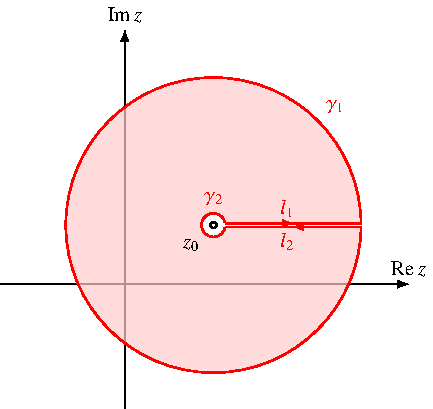
\includegraphics{chapters/080-funktionentheorie/images/laurent.pdf}
\caption{Pfad zur Herleitung der Laurent-Reihe einer Funktion $f(z)$
mit einer Singularität $z_0$.
\label{komplex:laurentpfad}}
\end{figure}%
\index{Laurent-Reihe}%
In Satz~\ref{komplex:integralanalytisch} konnten wir eine Potenzreihe für
solche $z$ konstruieren, deren Betrag kleiner ist als der kleinste Abstand
der Kurve $\gamma$ vom Ursprung.
Dies war notwendig, weil in~\eqref{komplex:georeihe} die geometrische Reihe
nur konvergiert, wenn der Quotient $<1$ ist.
Wenn die Funktion $f(z)$ jedoch eine Singularität im Punkt $z_0$ hat, dann
kann es nicht möglich sein, die Funktion mit einer Potenzreihe zu
beschreiben.

Wir verwenden daher den speziellen Pfad in Abbildung~\ref{komplex:laurentpfad}.
Er führt in einem grossen Kreis $\gamma_1$ um den Punkt $z_0$ herum,
dann folgt ein zur $x$-Achse paralleler Abschnitt, der bis zum kleinen
Kreis $\gamma_2$ führt.
Nach Durchlaufen des kleinen Kreises $\gamma_2$ im Uhrzeigersinn folgt wieder
ein zur $x$-Achse paralleles Stück zurück zum grossen Kreis.
Da die geraden Stücke zweimal in entgegegengesetzer Richtung durchlaufen
werden, heben sie sich weg.
Ein Wegintegral entlang $\gamma$ zerfällt daher in eine Differenz
\[
\oint_\gamma\dots\,dz
=
\oint_{\gamma_1}\dots\,dz
-
\oint_{\gamma_2}\dots\,dz
\]
von Wegintegralen entlang $\gamma_1$ und $\gamma_2$.

Der äussere Pfad $\gamma_1$ gibt wie in Satz~\ref{komplex:integralanalytisch}
Anlass zu einer Potenzreihe in $(z-z_0)$.
Der innere Pfad $\gamma_2$ kann aber nicht so behandelt werden, da $z$ immer
weiter von $z_0$ entfernt als die Punkte auf $\gamma_2$.
Allerdings ist $|x/z| < 1$ für Punkte auf $\gamma_2$, wir müssen daher
die geometrische Reihe auf $x/z$ anwenden:
\begin{align*}
\frac{1}{x-z}
&=
\frac{1}{x-z_0-(z-z_0)}
=
\frac{1}{z-z_0}
\cdot
\frac{1}{\displaystyle\frac{x-z_0}{z-z_0}-1}
=
-\sum_{k=0}^\infty \frac{(x-z_0)^k}{(z-z_0)^{k+1}}.
\end{align*}
Das Integral entlang der Kurve $\gamma_2$ kann also als Reihe in $1/(z-z_0)$
entwickelt werden:
\begin{align*}
f_2(z)
&=
\frac{1}{2\pi i}\int_{\gamma_2} \frac{g(x)}{x-z}\,dx
=
\frac{1}{2\pi i}\int_{\gamma_2}\sum_{k=0}^\infty
\frac{(x-z_0)^k}{(z-z_0)^{k+1}}\,dx
\\
&=
\sum_{k=0}^\infty
\biggl(
\underbrace{\frac1{2\pi i}\int_{\gamma_2} (x-z_0)^kg(x)\,dx
}_{\displaystyle =d_{k+1}}
\biggr)
\frac1{(z-z_0)^{k+1}}
=\sum_{k=1}^\infty \frac{d_k}{(z-z_0)^k}.
\end{align*}
Zusammen mit der vom Integral entlang $\gamma_1$ herrührenden Reihe finden
wir den Satz
\begin{satz}
\label{komplex:laurentreihe}
Ist $g(z)$ eine entlang der Kurve $\gamma$ wie in
Abbildung~\ref{komplex:laurentpfad} definierte stetige Funktion, dann gilt
\[
f(z)=\frac1{2\pi i}\oint_{\gamma} \frac{f(x)}{x-z}\,dx
=
\sum_{k=0}^{\infty} c_k(z-z_0)^k-\sum_{k=1}^\infty \frac{d_k}{(z-z_0)^k},
\]
wobei die Koeffizienten $c_k$ und $d_k$ gegeben sind durch
\[
\begin{aligned}
c_k&=\frac1{2\pi i}\oint_{\gamma_1} \frac{g(x)}{x-z_0}\,dx
&&
\text{und}
&
d_k&=\frac1{2\pi i}\oint_{\gamma_2} g(x)x^{k-1}\,dx.
\end{aligned}
\]
\end{satz}

\begin{definition}
Eine Reihe der Form
\[
\sum_{k=-\infty}^\infty a_k(z-z_0)^k
\]
heisst {\em Laurent-Reihe }
im Punkt $z_0$.
\end{definition}


%
% Geschlossene Wege
%
\subsubsection{Geschlossene Wege}
\begin{definition}
Ein Weg $\gamma\colon[a,b]\to\mathbb C$ heisst {\em geschlossen}, wenn
$\gamma(a)=\gamma(b)$.
\index{geschlossener Weg}
Das Integral entlang eines geschlossenen Weges hängt nicht von der
Parametrisierung ab und wird zur Verdeutlichung mit
\[
\int_{\gamma}f(z)\,dz
=
\oint_{\gamma}f(z)\,dz
\]
bezeichnet.
\end{definition}

\begin{beispiel}
Wir berechnen das Integral von $f(z)=z^n$ entlang des Einheitskreises,
den wir mit $\gamma(t)=e^{it},t\in[0,2\pi]$ parametrisieren.
Die Definition liefert:
\begin{align*}
\oint_{\gamma}f(z)\,dz
&=
\int_0^{2\pi}e^{int}ie^{it}\,dt
=
i\int_0^{2\pi}e^{i(n+1)t}\,dt
\end{align*}
Für $n=-1$ ist dies das Integral einer konstanten Funktion, also
\[
\oint_{\gamma}\frac1z\,dz=2\pi i.
\]
Für $n\ne -1$ kann man eine Stammfunktion von $e^{i(n+1)t}$
verwenden:
\[
\oint_{\gamma}f(z)\,dz
=
i\left[\frac1{i(n+1)}e^{i(n+1)t}\right]_0^{2\pi}
=0,
\]
weil $e^{i(n+1)t}$ periodisch ist mit Periode $2\pi$.
\end{beispiel}
Das Beispiel zeigt, dass ein Wegintegral der Potenzfunktionen,
aller Polynome und schliesslich aller konvergenten Potenzreihen
über einen geschlossenen Weg verschwinden.
Es zeigt aber auch, dass das Wegintegral über einen geschlossenen
Weg nicht zu verschwinden braucht, wie das Beispiel $f(z)=1/z$
zeigt.
Letztere Funktion unterscheidet sich von den Potenzfunktionen allerdings
dadurch, dass sie im Nullpunkt nicht definiert ist.

\begin{satz}
Sei $f(z)$ eine in einem zusammenhängenden Gebiet $\Omega\subset\mathbb C$
definierte komplexe Funktion, für die das Wegintegral über jeden
geschlossenen Weg verschwindet.
Dann hat $f(z)$ eine komplexe Stammfunktion $F(z)$.
\end{satz}

\begin{proof}[Beweis]
Wir wählen einen beliebigen Punkt $z_0\in\Omega$ definieren die
komplexe Stammfunktion mit Hilfe des Wegintegrals
\[
F(z)=\int_{\gamma_z} f(\zeta)\,d\zeta,
\]
wobei $\gamma_z$ ein beliebiger Weg ist, der $z_0$ mit $z$ verbindet.

Wir müssen uns davon überzeugen, dass die Wahl des Weges keinen Einfluss
auf $F(z)$ hat.
Dazu seien $\gamma_1$ und $\gamma_2$ zwei verschiedene Wege, die
$z_0$ mit $z$ verbinden.
Da die Parametrisierung der Wege keinen Einfluss auf das Wegintegral haben,
nehmen wir an, dass beide Wege auf dem Intervall $[0,1]$ definiert sind.

Jetzt konstruieren wir einen geschlossene Weg $\gamma$ durch die
Definition:
\[
\gamma\colon[0,2]\to\mathbb C:t\mapsto
\begin{cases}
\gamma_1(t)&\qquad 0\le t\le 1\\
\gamma_2(2-t)&\qquad 1\le t\le 2
\end{cases}
\]
Der Weg $\gamma$ besteht aus $\gamma_1$ und dem in umgekehrter Richtung
durchlaufenen Weg $\gamma_2$, denn an der Stelle $t=1$ passen die
beiden Teilwege nahtlos zusammen: $\gamma_1(1)=\gamma_2(1)=\gamma_2(2-1)$.
Wegen $\gamma(2)=\gamma_2(2-2)=\gamma_2(0)=\gamma_1(0)$ ist der
Weg geschlossen.
Nach Voraussetzung ist verschwindet das Wegintegral über $\gamma$.
Es folgt
\begin{align*}
0
&=
\int_{\gamma}f(z)\,dz
\\
&=
\int_0^1 f(\gamma_1(t))\gamma_1'(t)\,dt
+ \int_1^2f(\gamma_2(2-t))\frac{d}{dt}\gamma_2(2-t)\,dt
\\
&=
\int_0^1 f(\gamma_1(t))\gamma_1'(t)\,dt
- \int_1^2f(\gamma_2(2-t))\gamma_2'(2-t)\,dt
\\
&=
\int_0^1 f(\gamma_1(t))\gamma_1'(t)\,dt
- \int_0^1f(\gamma_2(s))\gamma_2'(s)\,ds
\\
&=
\int_{\gamma_1}f(z)\,dz - \int_{\gamma_2}f(z)\,dz
\\
\Rightarrow\qquad
\int_{\gamma_2}f(z)\,dz&=\int_{\gamma_1}f(z)\,dz.
\end{align*}
Da die Wahl des Weges keine Rolle spielt, ist $F(z)$ wohldefiniert.
\end{proof}

Die Bedingung des eben bewiesenen Satzes ist nicht wirklich nützlich,
sie ist kaum nachprüfbar.
Es braucht also zusätzliche Anstrengungen um genügend viele
Funktionen zu finden, welche die Eigenschaft haben, dass Wegintegrale
über geschlossene Wege verschwinden.
Wir zielen dabei auf den folgenden Satz hin:
\begin{satz}[Cauchy]
Ist $f(z)$ eine in einem Gebiet $\Omega\subset\mathbb C$ definierte
komplex differenzierbare Funktion, und ist $\gamma$ ein im Gebiet
$\Omega$ auf einen Punkt zusammenziehbarer geschlossener Weg, dann gilt
\[
\oint_{\gamma}f(z)\,dz=0.
\]
Ist insbesondere $\Omega$ {\em einfach zusammenhängend}
\index{einfach zusammenhangend@einfach zusammenhängend}%
\index{zusammenziehbar}%
(d.~h.~jeder geschlossene Weg lässt sich in einen Punkt zusammenziehen),
dann verschwindet das Wegintegral von $f(z)$ über jeden geschlossenen
Weg in $\Omega$.
\index{einfach zusammenhangend@einfach zusammenhängend}
\end{satz}


\begin{proof}[Beweis]
Wir verwenden für den folgenden Beweis den Satz von Green über
\index{Green, Satz von}%
Wegintegrale in der Ebene.
Er besagt, dass für einen geschlossenen Weg $\gamma$ der in der Ebene
das Gebiet $D$ berandet, und zwei Funktionen $L(x,y)$ und $M(x,y)$, gilt
\[
\oint_\gamma(L\,dx + M\,dy)
=
\int_D \biggl(\frac{\partial M}{\partial x}
-\frac{\partial L}{\partial y}\biggr)\,dx\,dy.
\]
Wir berechnen jetzt das Integral einer komplex differenzierbaren Funktion
$f(z)$
\begin{align*}
\oint_\gamma f(z)\,dz
&=
\int (u(x,y)+iv(x,y))(\dot x(t)+i\dot y(t))\,dt
\\
&=
\int u(x,y)\dot x(t) -v(x,y)\dot y(t)\,dt
+
i \int u(x,y)\dot y(t)+v(x,y)\dot x(t)\,dt
\\
&=\oint_\gamma(u\,dx - v\,dy) + i\oint_\gamma(v\,dx + u\,dy)
\\
&=
\int_D
\underbrace{-\frac{\partial v}{\partial x}}_{\displaystyle=\frac{\partial u}{\partial y}}
-\frac{\partial u}{\partial y}
\,dx\,dy
+i
\int_D
\underbrace{\frac{\partial u}{\partial x}}_{\displaystyle=\frac{\partial v}{\partial y}}
-\frac{\partial v}{\partial y}\,dx\,dy
=0.
\end{align*}
Dabei haben wir auf der dritten Zeile den Satz von Green angewendet,
und auf der letzten Zeile die Cauchy-Riemann-Differentialgleichungen.
\end{proof}

\subsection{Die Cauchy-Integralformel}
\index{Cauchy-Integralformel}%
Sei jetzt $f(z)$ eine komplex differenzierbare Funktion.
Dann ist auch die Funktion
\[
g(z)=\frac{f(z)}{z-a}
\]
komplex differenzierbar für $z\ne a$.
Insbesondere ist der Wert des Wegintegrals von $g(z)$ entlang
eines geschlossenen Pfades um den Punkt $a$ unabhängig von der Wahl
des Weges.
Zum Beispiel könnten wir das Wegintegral mit Hilfe eines kleinen Kreises
um $a$ mit Radius $r$ mit der Parametrisierung
\[
t\mapsto \gamma(t)=a+re^{it},\quad t\in[0,2\pi]
\]
berechnen.
Die Rechnung ergibt
\begin{align*}
\oint_\gamma \frac{f(z)}{z-a}\,dz
&=
\int_0^{2\pi} \frac{f(a+re^{it})}{re^{it}}ire^{it}\,dt
=
i\int_0^{2\pi} f(a+re^{it})\,dt
\end{align*}
Da $f(z)$ komplex differenzierbar ist, können wir $f(z)$ approximieren
durch $f(z)=f(a)+f'(a)(z-a)+o(z-a)$, also
\begin{align*}
\oint_{\gamma} \frac{f(z)}{z-a}\,dz
&=
i\int_0^{2\pi}f(a) + f'(a)re^{it}+o(r)\,dt
\\
&=
f(a)i\int_0^{2\pi}\,dt
+ irf'(a)\int_0^{2\pi} e^{it}\,dt + i\int_0^{2\pi}o(r)\,dt
\\
&=
2\pi i f(a) + irf'(a)\underbrace{\left[\frac1{i}e^{it}\right]_0^{2\pi}}_{\displaystyle=0}+o(r)
\\
&=2\pi i f(a)+o(r).
\end{align*}
Da das Wegintegral einer komplex differenzierbaren Funktion aber unabhängig
vom Weg und damit vom Radius $r$ sein muss, folgt
\[
\oint_\gamma \frac{f(z)}{z-a}\,dz=2\pi i f(a).
\]
Wir haben damit den folgenden Satz bewiesen:

\begin{satz}[Cauchy]
Ist $\gamma$ ein geschlossener Weg in der komplexen Ebene, die ein
Gebiet umrandet, in dem die komplexe Funktion $f(z)$ komplex
differenzierbar ist, dann gilt
\[
f(a)=\frac{1}{2\pi i}\oint_{\gamma}\frac{f(z)}{z-a}\,dz.
\]
Insbesondere sind die Werte einer komplex differenzierbaren Funktion
im Inneren eines Gebietes durch die Werte auf dem Rand bereits vollständig
bestimmt.
\end{satz}

\subsubsection{Ableitungen und Cauchy-Formel}
Sei $f(z)$ eine komplex differenzierbare Funktion, als Definitionsgebiet
nehmen wir der Einfachheit halber einen Kreis vom Radius $r$ um den Nullpunkt,
sein Rand ist die Kurve $\gamma$.
Durch Ableiten der Cachyschen Integralformel finden wir
\begin{align*}
f(z)
&=
\frac1{2\pi i}\oint_{\gamma}\frac{f(\zeta)}{\zeta-z}\,d\zeta
\\
f'(z)
&=
\frac1{2\pi i}\oint_{\gamma}\frac{f(\zeta)}{(\zeta-z)^2}\,d\zeta
\\
f'' (z)
&=
\frac1{2\pi i}\oint_{\gamma}2\frac{f(\zeta)}{(\zeta-z)^3}\,d\zeta
\\
f'''(z)
&=
\frac1{2\pi i}\oint_{\gamma}2\cdot 3\frac{f(\zeta)}{(\zeta-z)^4}\,d\zeta
\\
&\vdots
\\
f^{(k)}(z)
&=
\frac{k!}{2\pi i}\oint_{\gamma}\frac{f(\zeta)}{(\zeta-z)^{k+1}}\,d\zeta.
\end{align*}
Es folgt

\begin{satz}
Eine komplex differenzierbare Funktion ist beliebig oft differenzierbar.
\end{satz}

\subsubsection{Komplex differenzierbare Funktionen sind analytisch}
Wir haben früher gesehen, dass Wegintegrale auf analytische Funktionen
führen.
Andererseits zeigt das Cauchy-Integral, dass komplex differenzierbare
Funktionen durch genau die Integrale bestimmt sind, die in den
Reihenentwicklungen in Satz~\ref{komplex:integralanalytisch} auftraten.
Diese Resultate können wir im folgenden Satz zusammenfassen.

\begin{satz}
Eine komplex differenzierbare Funktion $f(z)$, die in einer Kreisscheibe
vom Radius $r$ um den Punkt $z_0$ definiert ist, ist analytisch.
Ihre Potenzreihenentwicklung
\[
f(z)=\sum_{k=0}^na_k(z-z_0)^k
\]
hat die Koeffizienten
\[
a_k=\frac1{2\pi i}\int_{\gamma}\frac{f(z)}{(z-z_0)^{k+1}}\,dz,\quad
k\ge 0.
\]
\end{satz}

\begin{proof}[Beweis]
Da $f$ komplex differenzierbar ist, gilt
\[
f(z)=\frac1{2\pi i}\oint_\gamma \frac{f(\zeta)}{\zeta-z}\,d\zeta.
\]
In Satz~\ref{komplex:integralanalytisch} wurde gezeigt, dass $f(z)$
analytisch ist, und dass die Koeffizienten der Potenzreihe von
der verlangten Form sind.
\end{proof}

Für eine komplexe Funktion, die im Punkt $z_0$ eine Singularität hat,
also in einer Umgebung von $z_0$ ohne den Punkt $z_0$ definiert ist,
können wir das Resultat aus Satz~\ref{komplex:laurentreihe} verwenden,
und zum folgenden analogen Resultat gelangen:

\begin{satz}
Eine komplex differenzierbare Funktion $f(z)$, die in einer Kreisscheibe
vom Radius $r$ um den Punkt $z_0$ mit Ausnahme des Punktes $z_0$
definiert ist, kann in eine konvergente Laurent-Reihe
\[
f(z)=\sum_{k=-\infty}^{\infty} c_k(z-z_0)^k
\]
entwickelt werden, deren Koeffizienten durch
\[
c_k = \frac1{2\pi i}\oint_\gamma \frac{f(\zeta)}{(z-z_0)^{k+1}}\,d\zeta,\qquad k\in\mathbb Z
\]
gegeben sind.
\end{satz}

